\chapter{Related Works}\label{ch:related_works}
This thesis builds upon prior research in \ac{KG} fact verification, \ac{LLMs}, \ac{RAG}, and entailment verification.
In this section, we provide an overview of the relevant literature across these areas.
We categorized them into different sections based on their relevance to the proposed work.

\section{\ac{KG} and Fact-Checking}\label{sec:knowledge-graph-fact-verification}
\acp{KG} can involve in the Fact-Checking task in two ways:
(1) Using KG structured data to verify the data or facts
and (2) Using the structured or unstructured information to verify the information inside the KG triples.
\paragraph{Fact-Checking using KG Structured Data:}
By exploiting the structured data in the KG, we can find that whether the claim (\ie text) is correct or not.
For example for finding if a person is father of another person, the first step is checking the relations like \textit{fatherOf} in the KG or checking.
Afterward we can check the relations like \textit{birthdate} to find the age of the person as the father should be older than the child.
As our purpose is to verify the facts in the KG, this approach is out of the scope of this thesis.

\paragraph{KG Fact-Checking using External Data:}
We focus on the KG fact checking approach, where we use the unstructured information from exteranl sources to verify the information inside the triples.

\subsection{DeFacto}\label{subsec:defacto}
DeFacto~\cite{GERBER201585} is designed to check if facts are true by finding supporting evidence on the web.
What makes DeFacto special is that it works in multiple languages and can determine when facts were true.

Gerber et al.~\cite{GERBER201585} created a system that takes a fact (in RDF triple format) and searches the web for evidence that confirms it.
DeFacto looks for mentions of the fact in English, German, and French websites.
It then calculates a confidence score to tell users how likely the fact is to be true.
The system also tries to figure out the time period when the fact was valid.
DeFacto first converts the fact into natural language patterns that might appear on websites.
It then searches the web using these patterns and analyzes the returned pages for confirming text.
The system also considers how trustworthy each website is.
For the time aspect, DeFacto looks for year mentions near where the fact is discussed.
It uses patterns and frequency analysis to determine when a fact was valid.
This is important because many facts are only true during specific time periods.

Gerber et al. tested DeFacto on a dataset they created called \textit{FactBench}, which contains 1,500 facts across 10 different types of relations (like births, deaths, marriages, etc.).
Their results showed that DeFacto achieves about 85\% accuracy in determining if facts are true.
For figuring out when facts were true, the accuracy was around 70\% for simple time points and 66\% for time periods.
One important finding was that using multiple languages improved performance significantly.
By combining evidence from English, German, and French websites, DeFacto performed better than when using only English.

Our work has some intersection with DeFacto, but there are some key differences.
The intersection is as follows:
(1) we use web search to verify facts.
We feed the web search results as context to the \ac{LLMs} to verify the facts.
and additionally, (2) We use the dataset that they created (\ie FactBench) to evaluate our system.
The differences are as follows:
(1) We use \ac{LLMs} to verify the facts.
(2) We use the \ac{RAG} technique to retrieve the evidence and
(3) we use the ensemble of \ac{LLMs} to verify the facts to have more reliable results.

\subsection{Validating RDF Triples Using Textual Evidence}\label{subsec:validating-rdf-triples-using-textual-evidence}
Syed et al.~\cite{10.1145/3269206.3269308} introduces a new approach for automatically validating facts in \acp{KG}.
They present a system that improves upon existing fact validation methods by combining deep sentence parsing with topic coherence analysis to evaluate the truthfulness of RDF triples based on textual evidence from reference corpora.
This represents a significant advancement over previous approaches like DeFacto (\S\ref{subsec:defacto}), which relied primarily on string matching and word proximity.
The system architecture follows a systematic process: First, input RDF triples are verbalized into natural language statements.
These verbalizations are used to search reference corpora (either Wikipedia or ClueWeb) for supporting textual evidence.
For each piece of evidence, the system extracts features through dependency parsing to identify direct relationships between subject, predicate, and object.
Additionally, it calculates topic coherence values to measure the semantic relatedness of terms.
These features, along with others shared with DeFacto, serve as input to machine learning classifiers that determine a confidence score for each triple.

The authors also analyzed the impact of corpus size, finding that larger reference corpora improved performance for both systems.
Feature analysis confirmed the importance of the newly introduced dependency parsing and topic coherence features in achieving these performance gains.

The system still relies on the presence of explicit textual evidence in the reference corpora, and the computational complexity of dependency parsing could pose scalability challenges for very large knowledge bases.
The paper also doesn't extensively discuss how the system handles more complex or composite facts.
In our work, we address these limitations by leveraging \ac{LLMs} to verify facts in knowledge graphs, which can handle more complex reasoning tasks and provide more nuanced assessments of fact veracity.
Also, we do the similar analysis on the impact of the corpus size and the features used in the system for the \textit{DBpedia} dataset.


\section{LLMs and Retrieval-Augmented Generation}\label{sec:llms-and-retrieval-augmented-generation}
In this section we will discuss the related works on \ac{LLMs} and \ac{RAG} for general fact-verification task.
Eventually, in the \S~\ref{subsec:rag-base-systems-best-practices} we will discuss the best practices for the \ac{RAG} based systems.

\subsection{Entailment Verification and Language Models}\label{subsec:entailment-verification}
In the paper ``Minds versus Machines: Rethinking Entailment Verification with Language Models'', Sanyal et al.~\cite{sanyal2024machinesbettercomplexreasoning} evaluate and compare the inference capabilities of humans and \ac{LLMs} through a carefully constructed entailment verification benchmark.
Their study spans three categories: \ac{NLI}, contextual \ac{QA}, and rationales, using multi-sentence premises and diverse types of knowledge to assess inference across complex reasoning scenarios.
The authors found that LLMs generally excel in multi-hop reasoning tasks, particularly those requiring inference over extended contexts, while humans outperform \acp{LLM} in simpler deductive reasoning tasks involving substitutions or negations.

\begin{figure}[ht!]
    \centering
    \begin{minipage}[b]{\textwidth}
        \centering
        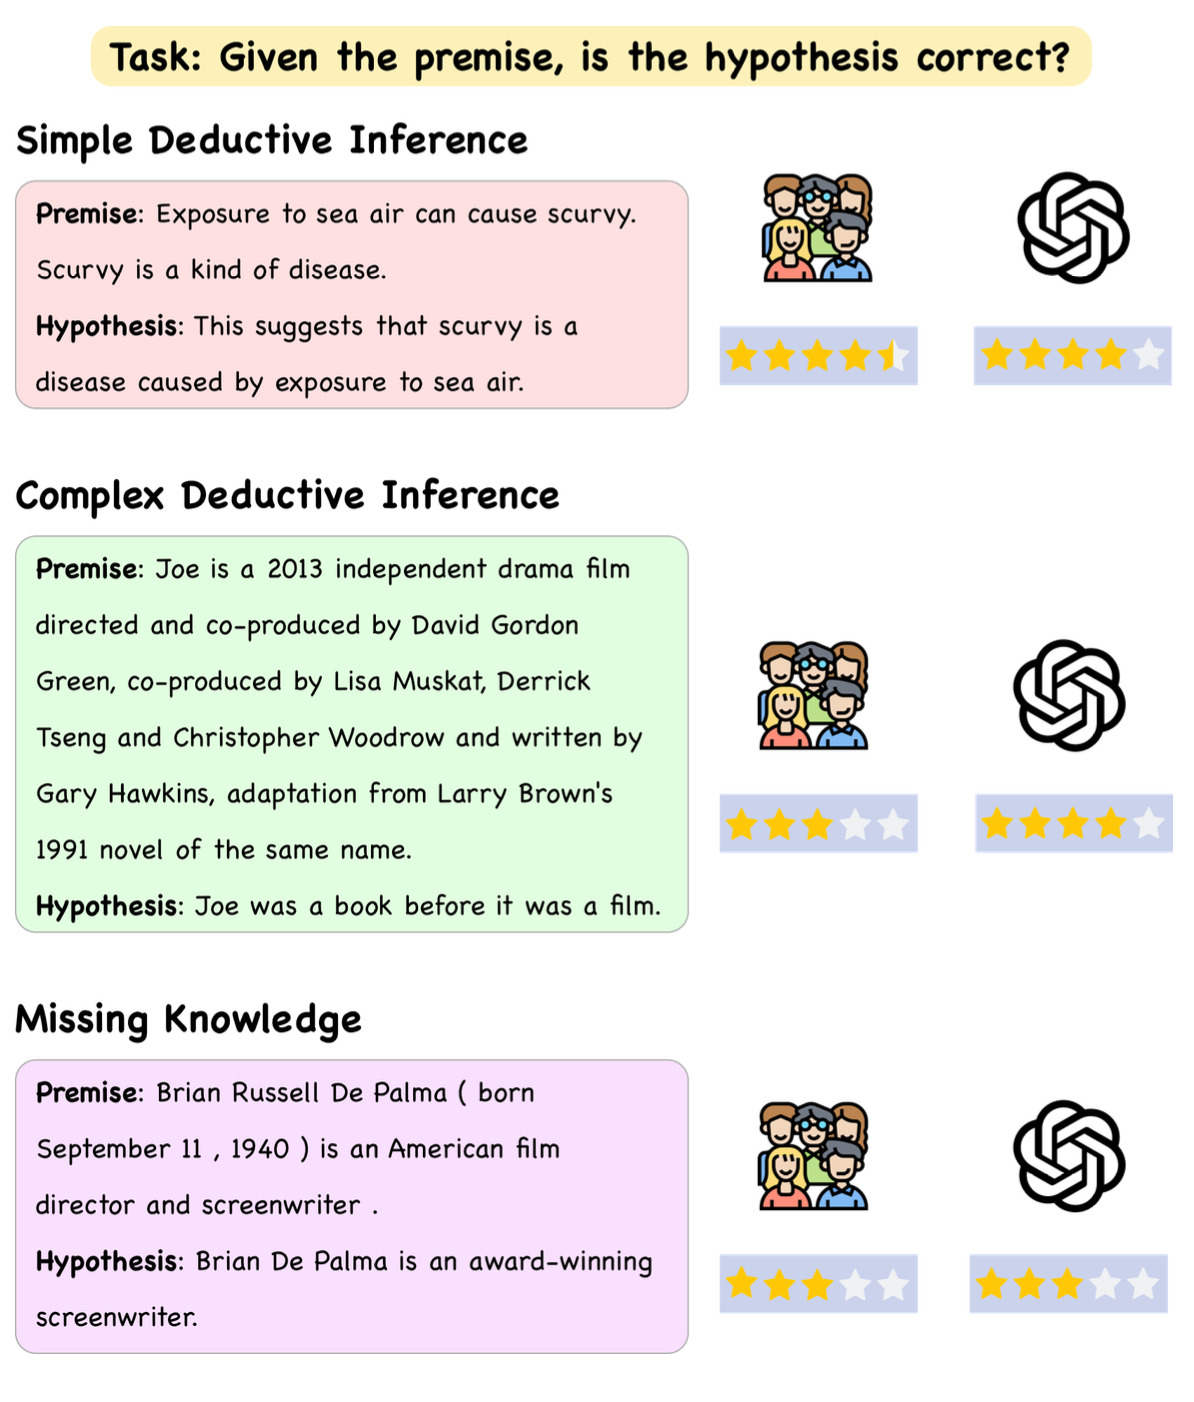
\includegraphics[width=0.6\textwidth]{res/rel-human-llm-inference}
    \end{minipage}
    \caption{Distinctions between human and LLM Inferences. The entailment prediction performance of humans and LLMs are depicted by a 5-star rating scale~\cite{sanyal2024machinesbettercomplexreasoning}.}
    \label{fig:distinguishing-human-llm-inferences}
\end{figure}

Interestingly, both perform comparably in situations requiring inference of missing knowledge.
One of the paper's key contributions is the fine-tuning of the Flan-T5~\cite{https://doi.org/10.48550/arxiv.2210.11416} model, which outperforms GPT-3.5 and performs at a comparable level to GPT-4, thus providing a robust, open-source solution for entailment verification tasks.
In contrast, the proposed approach to factulizing the knowledge graph using \ac{RAG} emphasizes the integration of external knowledge retrieval to ground factual assertions, which is critical for generating verifiable, accurate knowledge graphs.
While Sanyal et al. focus on the entailment between premises and hypotheses in textual inference, my work extends this by incorporating external evidence to ensure not just consistency but also factual correctness.

In comparison, the entailment verification tasks handled by Sanyal et al. emphasize reasoning within the constraints of the given context, whereas my \ac{RAG}-based approach highlights the necessity of retrieval from large external datasets to mitigate hallucinations and improve the factual grounding of generated content.
Both approaches deal with inference verification but diverge in their method of contextualizing and validating knowledge, with mine incorporating real-time retrieval for fact-checking.

This distinction is significant in terms of application: while their fine-tuned Flan-T5 model achieves high accuracy in entailment tasks, it remains bound to the contextual limits of its training data.
My work, by integrating retrieval, potentially overcomes this limitation by dynamically accessing external data, thus offering a complementary perspective to entailment verification focused on enhancing factuality.

\subsection{Claim Verification in the Age of Large Language Models}\label{subsec:claim-verification-in-the-age-of-large-language-models}
Dmonte et al.~\cite{dmonte2024claimverificationagelarge} provide a comprehensive survey of \ac{LLM}-based approaches to claim verification, highlighting the shift from traditional \ac{NLP} methods to more sophisticated LLM-driven techniques.
The typical LLM-based claim verification pipeline, as described by Dmonte et al., consists of several key components:
(1) \textbf{Evidence Retrieval:} Utilizing techniques like \ac{RAG} to fetch relevant information from external sources;
(2) \textbf{Prompt Creation:} Developing effective prompting strategies to guide LLMs in processing claims and evidence;
(3) \textbf{Transfer Learning:} Employing fine-tuning and in-context learning to adapt LLMs to the specific task of claim verification;
and finally, (4) \textbf{LLM Generation:} Using LLMs to generate veracity labels, supporting evidence, and explanations.

This pipeline represents a departure from traditional fact-checking approaches, leveraging the power of \ac{LLMs} to improve accuracy and provide more nuanced assessments of claim veracity.
Based on survey, several studies have demonstrated the effectiveness of LLM-based approaches in claim verification:
\begin{itemize}
    \item Zhang and Gao~\cite{zhang2023llmbasedfactverificationnews} introduced the Hierarchical Step-by-Step (HiSS) prompting method, which directs LLMs to separate a claim into several sub-claims and then verify each via multiple questions-answering steps progressively, improving performance on complex news claim verification tasks.
    \item Lee et al.~\cite{lee2023factualityenhancedlanguagemodels} developed FactualityPrompts, a framework for assessing the factual accuracy of LLM-generated content.
\end{itemize}

These studies consistently show that LLM-based methods outperform traditional NLP approaches in terms of accuracy, flexibility, and the ability to handle complex claims.
\begin{figure}[ht!]
    \centering
    \begin{minipage}[b]{\textwidth}
        \centering
        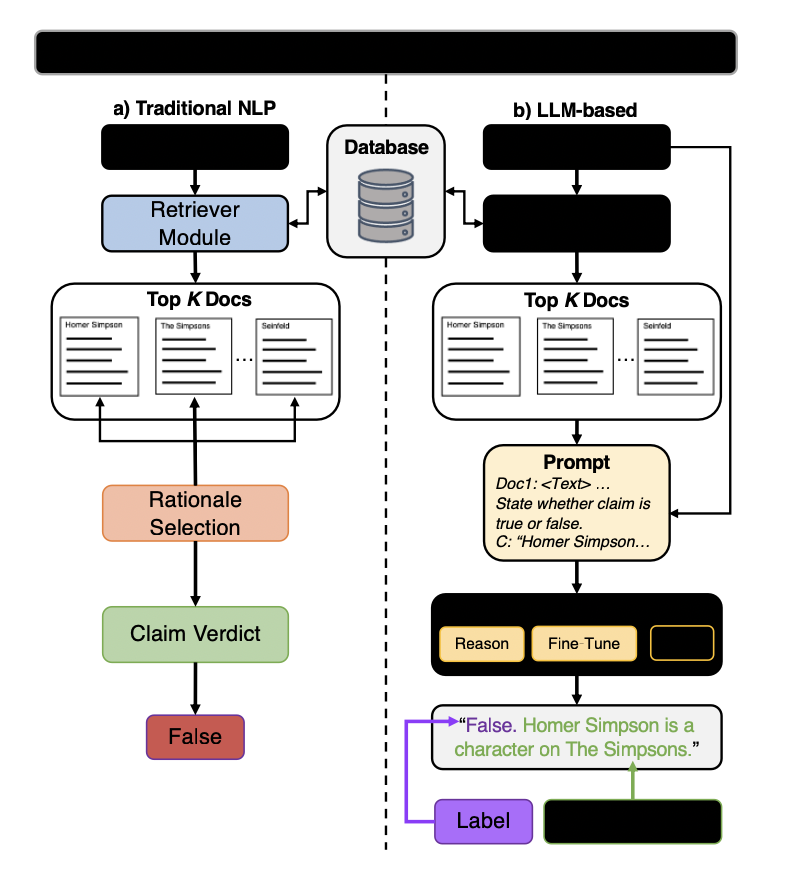
\includegraphics[width=0.6\textwidth]{res/rel-claim-verification}
    \end{minipage}
    \caption{Comparison of claim verification systems between NLP-based (traditional) and LLM-based for claim veracity~\cite{dmonte2024claimverificationagelarge}.}
    \label{fig:claim-verification-llm}
\end{figure}

Our approach shares similarities with the LLM-based pipeline described by Dmonte et al., particularly in the use of retrieval-augmented generation and the integration of multiple LLMs. However, our method differs in several key aspects:
\begin{enumerate}
    \item \textbf{Multi-Query Retrieval:} We employ a multi-query strategy for evidence retrieval, potentially improving the coverage and relevance of supporting information.
    \item \textbf{Iterative Refinement:} Our system incorporates an iterative process for refining retrieved evidence and generated responses, which is not explicitly mentioned in most LLM-based approaches surveyed.
    \item \textbf{Limited Explanation:} While many LLM approaches provide explanations, our method places a stronger emphasis on generating binary (pass/fail) labels for claims to reduce the costs of using LLMs.
    \item \textbf{Diverse LLM Model:} We use multiple LLMs with diverse architectures to provide more reliable verification result.
\end{enumerate}

These distinctions position our work as a new contribution to the field, building upon the foundations of LLM-based claim verification while introducing innovative techniques to enhance performance and interpretability.

Despite the promising results of LLM-based fact verification, several challenges remain.
Dmonte et al. highlight issues such as handling irrelevant context, resolving knowledge conflicts, and expanding to multilingual settings. Our approach attempts to address some of these challenges, particularly in the areas of context relevance and explainability. However, there is still significant room for improvement in creating more robust, reliable, and universally applicable claim verification systems.

\subsection{RAG-Based Fact Verification by Synthesizing Contrastive Arguments}\label{subsec:retrieval-augmented-fact-verification}
The paper Retrieval-Augmented Fact Verification by Synthesizing Contrastive Arguments~\cite{yue2024retrievalaugmentedfactverification} explores a method for improving fact verification in knowledge graphs using RAG.
The proposed framework combines retrieval of external information and the generation of contrastive arguments-claims supported by retrieved evidence, but also those that provide counterpoints.
This dual synthesis provides a richer and more nuanced verification process, allowing the system to handle conflicting evidence more effectively.
The core contribution of the work lies in the creation of contrastive arguments, a strategy designed to reduce errors in fact verification systems, especially when LLMs may hallucinate or generate incomplete reasoning.

The authors leverage a multi-stage pipeline where external documents are retrieved to support or refute a given claim.
Each retrieved piece of evidence is evaluated using a neural network model that ranks the evidence based on its relevance to the claim.
By synthesizing contrastive arguments, the system generates explanations for both supporting and refuting the claim, which helps improve the transparency and trustworthiness of the model's decisions.

\begin{figure}[ht!]
    \centering
    \begin{minipage}[b]{\textwidth}
        \centering
        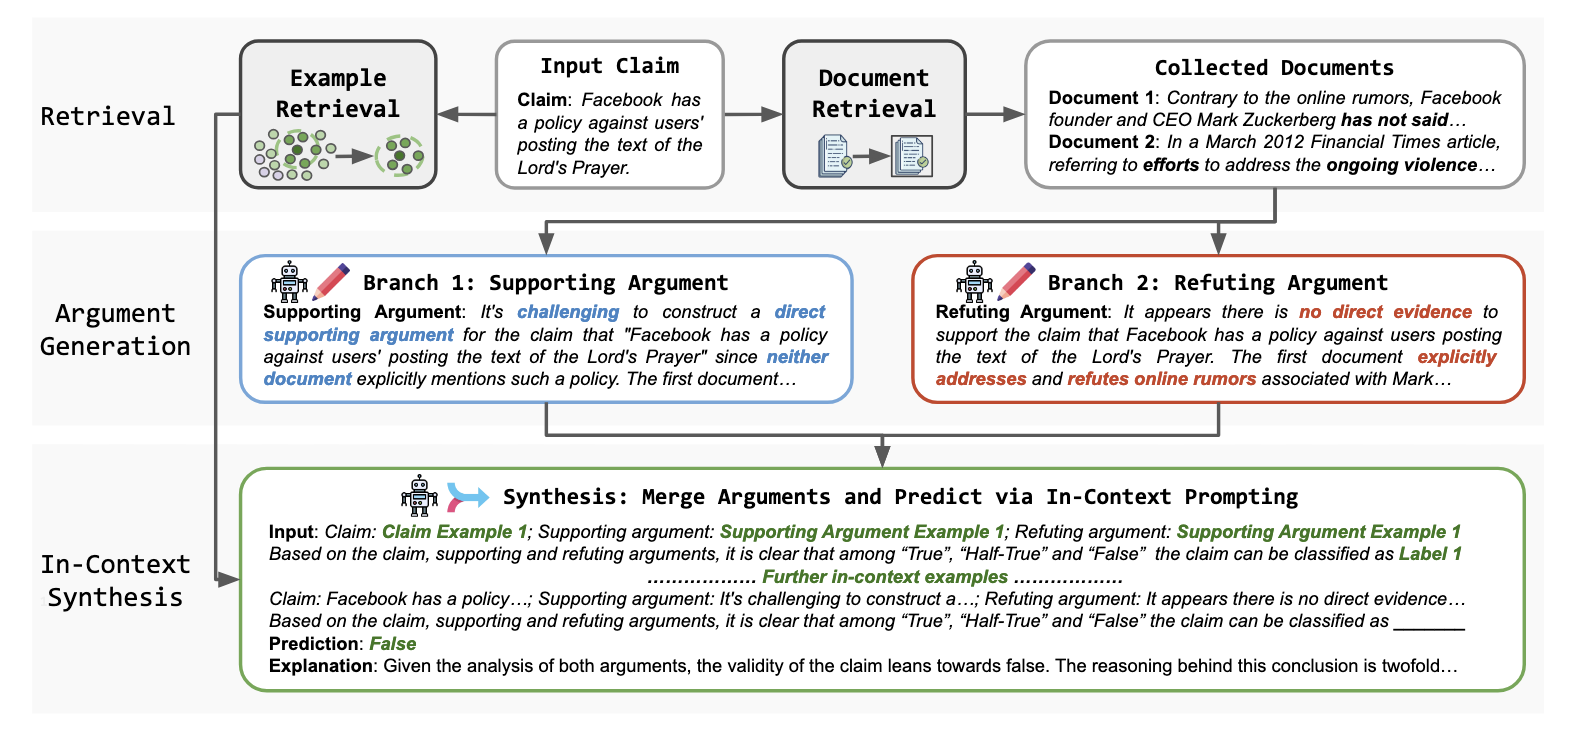
\includegraphics[width=\textwidth]{res/rel-rafts}
        \caption{The proposed RAFTS~\cite{yue2024retrievalaugmentedfactverification}, which performs few-shot fact verification by incorporating informative in-context demonstrations and contrastive arguments with nuanced information derived from the retrieved documents}
        \label{fig:rel-rafts}
    \end{minipage}
\end{figure}

In terms of results, the framework shows improvement over traditional fact verification pipelines, particularly in handling ambiguous or conflicting information.
The contrastive arguments allow for better handling of cases where facts are not binary but exist in a more complex, nuanced state.
The system's ability to generate arguments for both sides of a claim increases its robustness and provides a more reliable fact verification tool.

The described approach and my work on fact verification in knowledge graphs using RAG share a common goal: improving the factual accuracy of information through the integration of external knowledge retrieval.
However, there are key differences in the methodologies used.
The contrastive argument synthesis introduced by the authors focuses heavily on generating both supporting and opposing arguments for claims, which provides a more holistic perspective in scenarios where evidence is mixed.
In contrast, my approach emphasizes majority voting among multiple models and a multi-query strategy to retrieve a broader range of external evidence, aiming to reduce the incidence of hallucinations in LLM outputs.

While both approaches use retrieval to mitigate the limitations of LLMs, my work incorporates adaptive dispute resolution techniques and focuses on synthesizing outputs from multiple LLMs rather than generating contrastive arguments.
This means that my approach leans more towards optimizing model diversity and utilizing the best consensus from several LLMs to ensure factual accuracy, rather than explicitly generating opposing arguments for each claim.

\subsection{RAGAR: RAG-Augmented Reasoning for Political Fact-Checking using Multimodal LLMs}\label{sec:agar-rag-augmented-reasoning}
The study titled ``RAGAR: RAG-Augmented Reasoning for Political Fact-Checking using Multimodal LLMs''~\cite{khaliq2024ragarfalsehoodradarragaugmented} introduces a new methodology to political fact-checking by leveraging RAG with multimodal LLMs.
This work focuses on enhancing fact verification in the politically sensitive domain, where disinformation can have far-reaching consequences.
The authors integrate various modalities text, images, and other media sources into a unified fact-checking pipeline powered by LLMs, particularly emphasizing RAG’s ability to retrieve and synthesize external evidence to validate or refute claims.

\begin{figure}[ht!]
    \centering
    \begin{minipage}[b]{\textwidth}
        \centering
        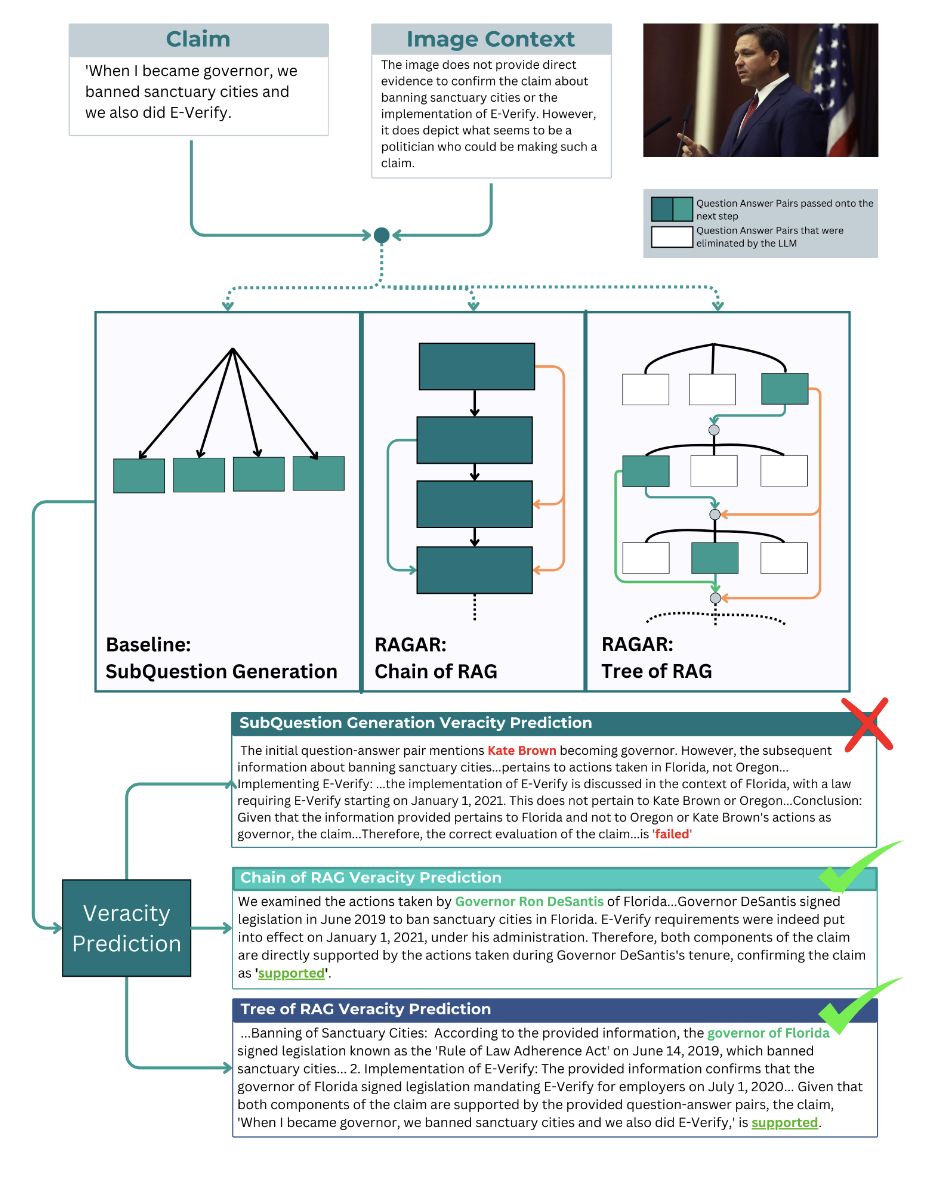
\includegraphics[width=0.6\textwidth]{res/rel-ragar}
    \end{minipage}
    \caption{An overview of the fact-checking pipeline contrasting the baseline Sub-Question Generation approach from the Chain of RAG and Tree of RAG approach followed by veracity prediction and explanation.}
    \label{fig:rel-ragar}
\end{figure}

The central innovation of RAGAR lies in its multimodal reasoning capabilities, which allow the model to handle political claims that involve not only textual content but also visual data, such as images or charts.
By extending RAG to this multimodal context, the system improves its ability to assess the veracity of claims in real-time, leveraging external resources such as political databases and live web content.
Furthermore, the use of contrastive learning helps the system generate both supporting and opposing arguments for each claim, providing a more balanced and comprehensive fact-checking process.

Results from the paper show significant improvements in fact-checking accuracy, particularly for politically charged claims that are often more nuanced or context-dependent.
RAGAR's ability to synthesize multimodal evidence into a coherent verification report highlights its potential for real-world applications, especially in environments where disinformation spreads quickly, such as social media platforms.

RAGAR focuses on political fact-checking using multimodal data, whereas my work targets the factualization of knowledge graphs with a primary focus on textual information.
In contrast to RAGAR’s multimodal pipeline, my system emphasizes multi-query strategies and document chunking techniques to retrieve highly relevant textual evidence for verification.

\subsection{Best Practices}\label{subsec:rag-base-systems-best-practices}
Different practices for \ac{RAG}-based systems have been explored in several recent studies for finding the best and optimal parameters/models for different components of the \ac{RAG} systems.
Studies~\cite{wang2024searchingbestpracticesretrievalaugmented, llamaindex_chunk_size} try to find the best practices for different \ac{RAG} components by examining the impact of different strategies on the performance of \ac{LLMs}.
These studies are evaluating different aspects of the RAG based system and provide detailed comparison between the components from the retrieval to the generation part of the system.

In the same way we try to conduct cold ablation study on fact verification task and provide detailed comparison between the components of the system.
Insights from these studies can help us choose initial parameters.
Our work also go beyond these studies by providing the timing analysis that help users to know the trade-offs.

\section{Cost Estimation}\label{sec:cost-estimation}
%TODO: CITE THE CYC, FREEBASE, DBPEDIA, YAGO, NELL
Heiko Paulheim~\cite{DBLP:conf/semweb/Paulheim18a} addresses an important yet underexplored aspect of \ac{KG} research: the economic cost of creating \acp{KG}.
While \acp{KG} have been extensively analyzed in terms of size, overlap, and quality, Paulheim provides a perspective by quantifying the financial investment required for both manual and automated \ac{KG} creation.
The author offers cost estimates for several well-known \acp{KG}.
For manually curated resources, Cyc~\cite{10.1145/219717.219745} costs approximately \$5.71 per statement (totaling \$120M for 21M assertions), while Freebase costs about \$2.25 per statement (\$6.75B total for 3B facts).
In contrast, automatically created \ac{KG} are substantially more cost-effective~\cite{One_Knowledge_Graph}: DBpedia costs only \$0.0125 per statement (\$5.1M development cost for 400M statements), YAGO costs \$0.0083 per statement (combining Wikipedia extraction with WordNet), and NELL costs \$0.1425 per statement.
The paper demonstrates that automatic \ac{KG} creation is approximately 15-250 times more cost-effective than manual curation, providing a clear economic argument for automation.
In general, We noticed that the manual curation of \acp{KG} is expensive and time-consuming, while automatic creation is more cost-effective and scalable.

Here, in this thesis we also provide the cost of using \acp{LLM} by providing the amount of tokens used for each model.
Through this we can estimate the cost of using \acp{LLM} for fact verification in \acp{KG}.
Additionally, we provide a time analysis of the models to estimate the time required to verify a fact in a \ac{KG} in the local infrastructure setup.